\DocumentMetadata{}
\documentclass[dvipsnames,12pt]{exam}
% compiles with: latexmk -pdflatex=lualatex -pdf exam.tex

\usepackage[top = 2cm, bottom = 3cm, left=1.5cm, right=1.5cm]{geometry}
\usepackage{microtype,fontspec,amssymb,titlesec,multicol,braket,graphicx,tikz,pgfplots}
\usepgfplotslibrary{fillbetween}
\usetikzlibrary{intersections,arrows.meta,decorations.pathreplacing}
\graphicspath{{./img/}}
\usepackage[shortlabels]{enumitem}
\usepackage{xcolor,cancel,amsmath,hyperref,eso-pic}
\runningfooter{}{}{\thepage}
\runningheader{}{}{\scriptsize Aayush Bajaj | z5362216}

\hypersetup{
  colorlinks   = true,
  linkcolor    = RedViolet,
  citecolor    = gray
}

\titleformat{\section}{\normalfont\Large\bfseries}{{\color{RedViolet}\S}}{0.5em}{}
\titleformat{\subsection}{\normalfont\large\bfseries}{{\large \color{RedViolet}\S\S}}{0.5em}{}
\titleformat{\subsubsection}{\normalfont\bfseries}{{\color{RedViolet}\S\S\S}}{0.5em}{}

\parindent 0pt
%%% defs
\newcommand{\N}{\mathbb{N}}
\newcommand{\C}{\mathbb{C}}
\newcommand{\D}{\mathbb{D}}
\newcommand{\F}{\mathcal{F}}
\renewcommand{\P}{\mathcal{P}} %careful
\newcommand{\R}{\mathbb{R}}
\newcommand{\Q}{\mathbb{Q}}
\newcommand{\T}{\mathbb{T}}
\newcommand{\Z}{\mathbb{Z}}
\newcommand{\ds}{\displaystyle}
\newcommand{\st}{\,:\,}
\newcommand{\norm}[1]{\Vert #1 \Vert}
\newcommand{\cl}{\mathop{\mathrm{cl}}}
\newcommand{\Int}{\mathop{\mathrm{Int}}}
%%% end defs

\usepackage{amsthm}
\newtheorem{theorem}{Theorem}[section]
\newtheorem{lemma}[theorem]{Lemma}
\newtheorem{prop}{Proposition}
\newtheorem{remark}{Remark}
\newtheorem{definition}{Definition}[section]

\AddToShipoutPictureBG*{
  \AtPageCenter{\makebox(0,0){\rotatebox{45}{\textcolor{gray!30}{\fontsize{70}{70}\selectfont Property of MATH3611}}}}
}

\author{Aayush Bajaj | z5362216}
\date{\today}
\title{MATH3611 --- Final Solutions}

% Toggle solutions:
\printanswers
%\noprintanswers

\begin{document}
\maketitle
\dotfill
\tableofcontents
\vspace{0.5cm}
\newpage

%%%%%%%%%%%%%%%%%%%%%%%%%%%%%%%%%%%%%%%%%%%%%%%%%%%%%%%%%%%%%%%%%%%%%%%%%%%%%%%%
% QUESTIONS
%%%%%%%%%%%%%%%%%%%%%%%%%%%%%%%%%%%%%%%%%%%%%%%%%%%%%%%%%%%%%%%%%%%%%%%%%%%%%%%%
\begin{questions}

%===============================================================================
\addcontentsline{toc}{section}{Q1. Set Theory}

\question[15] Set Theory

\begin{parts}
    \part[5] 
    \begin{subparts}
        \subpart $|A|\le |B|$
        \begin{solution}means there exists an \textbf{injective} map $f:A\to B$.\end{solution}

        \subpart $|A|=|B|$ 
        \begin{solution}means there exists a \textbf{bijective} map $f:A\to B$.\end{solution}

        \subpart $|A|<|B|$ 
        \begin{solution}means $\exists$ injective but not \textbf{surjective} map $A\to B$.\end{solution}

        \subpart Prove that $|\N| = |2\N|$.
        \begin{solution}
        Consider $f:\N\to 2\N$ given by $f(n)=2n$. It is clearly injective and surjective. The correspondence is illustrated below.

        \begin{center}
        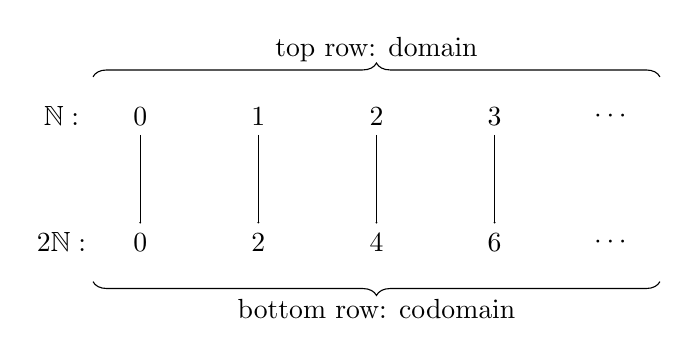
\begin{tikzpicture}[>=Latex, node distance=1.6cm]
          % top row: N
          \node (nlabel) at (-1.0,0) {$\N:$};
          \node (n0) at (0,0) {$0$};
          \node (n1) at (1.5,0) {$1$};
          \node (n2) at (3.0,0) {$2$};
          \node (n3) at (4.5,0) {$3$};
          \node (ndots) at (6.0,0) {$\cdots$};

          % bottom row: 2N
          \node (elabel) at (-1.0,-1.6) {$2\N:$};
          \node (e0) at (0,-1.6) {$0$};
          \node (e1) at (1.5,-1.6) {$2$};
          \node (e2) at (3.0,-1.6) {$4$};
          \node (e3) at (4.5,-1.6) {$6$};
          \node (edots) at (6.0,-1.6) {$\cdots$};

          % vertical “ladder” arrows (double-lined head via Implies)
          \draw[-{Implies[length=7pt]}] (n0) -- (e0);
          \draw[-{Implies[length=7pt]}] (n1) -- (e1);
          \draw[-{Implies[length=7pt]}] (n2) -- (e2);
          \draw[-{Implies[length=7pt]}] (n3) -- (e3);

          % braces for labels
          \draw[decorate,decoration={brace,amplitude=5pt}] (-0.6,0.5) -- (6.6,0.5)
            node[midway, yshift=10pt]{top row: domain};
          \draw[decorate,decoration={brace,mirror,amplitude=5pt}] (-0.6,-2.1) -- (6.6,-2.1)
            node[midway, yshift=-10pt]{bottom row: codomain};
        \end{tikzpicture}
        \end{center}

        Thus $f$ is a bijection and $|\N|=|2\N|$.
        \end{solution}
    \end{subparts}

    \part[10]
    \begin{subparts}
        \subpart State the Schroder--Bernstein Theorem. This is also known as the Cantor Bernstein Theorem.
        \begin{solution}
          If $|A|\le|B|$ and $|B|\le|A|$ then $|A|=|B|$.
        \end{solution}

        \subpart If $A$ is infinite, show $|\N|\le|A|$.
        \begin{solution}
          Pick distinct $a_0,a_1,\dots\in A$ recursively; $n\mapsto a_n$ is injective $\N\hookrightarrow A$.
        \end{solution}

        \subpart Deduce $|A\cup\N|=|A|$ for infinite $A$.
        \begin{solution}
          Trivially $|A|\le|A\cup\N|$. From (b) get injection $\N\hookrightarrow A$; combine with inclusion $A\hookrightarrow A$ to build an injection $A\cup\N\hookrightarrow A$ by sending $n\mapsto a_{2n+1}$ and $a_k\mapsto a_{2k}$. Apply Schröder--Bernstein.
        \end{solution}

        \subpart If $A$ is countably infinite prove that $|\N| \leq |A|$.
        \begin{solution}
          Since $A$ is countably infinite, there exists a bijection $h:\N\to A$, hence a fortiori an injection $\N\hookrightarrow A$. Therefore $|\N|\le |A|$.
        \end{solution}
    \end{subparts}
\end{parts}

%===============================================================================
\addcontentsline{toc}{section}{Q2. Metric Spaces}

\question[13] Metric Spaces
\begin{parts}
    \part Define a Metric Space $(X,d)$.
    \begin{solution}
      A metric space is a set $X$ with $d:X\times X\to[0,\infty)$ such that for all $x,y,z\in X$:
      \[
      d(x,y)=0\iff x=y,\quad d(x,y)=d(y,x),\quad d(x,z)\le d(x,y)+d(y,z).
      \]
    \end{solution}

    \part Define an open set $Y\subseteq X$.
    \begin{solution}
      $U\subseteq X$ is open if for each $x\in U$ there exists $r>0$ with the open ball $B(x,r)=\{y\in X: d(x,y)<r\}\subseteq U$.
    \end{solution}

    \part Define a boundary point.
    \begin{solution}
      A point $x\in X$ is a \emph{boundary point} of $A\subseteq X$ if every open ball $B(x,r)$ meets both $A$ and $X\setminus A$. The boundary is $\partial A=\cl(A)\setminus \Int(A)$.
    \end{solution}

    \part[4] Prove that the interior of $Y$ is open.
    \begin{solution}
      By definition,
      \[
        \Int(Y)=\bigcup\{\,B(x,r): x\in Y,\ r>0,\ B(x,r)\subseteq Y\,\},
      \]
      a union of open balls. Unions of open sets are open, so $\Int(Y)$ is open.
    \end{solution}
\end{parts}

%===============================================================================

\addcontentsline{toc}{section}{Q3. Sequences}

\question[5] Suppose $\limsup x_n=a$ and $\limsup x_n=b$. Prove $a=b$.
\begin{solution}
  Assume $a<b$ and set $\varepsilon=\frac{b-a}{3}$. By the $\limsup$ characterization, eventually $x_n<a+\varepsilon$, but for infinitely many $n$, $x_n>b-\varepsilon$. Thus for some $n$,
  \[
    b-\varepsilon<x_n<a+\varepsilon \ \Rightarrow\ b-a<2\varepsilon=\tfrac{2}{3}(b-a),
  \]
  a contradiction. Symmetrically $b\le a$. Hence $a=b$.
\end{solution}

%===============================================================================
\addcontentsline{toc}{section}{Q4. Norm Topology}

\question[11] Norm Topology

\begin{parts}
    \part Define a Normed Space.
    \begin{solution}
      A normed space is a vector space $V$ over $\R$ or $\C$ with $\|\cdot\|:V\to[0,\infty)$ such that for all $x,y\in V$, $\alpha$ scalar:
      \[
        \|x\|=0\iff x=0,\quad \|\alpha x\|=|\alpha|\,\|x\|,\quad \|x+y\|\le \|x\|+\|y\|.
      \]
    \end{solution}

    \part Define a Banach Space.
    \begin{solution}
      A Banach space is a complete normed space, i.e.\ every Cauchy sequence converges in norm to a limit in the space.
    \end{solution}

    \part Consider a Cauchy sequence $(f_n)_{n\ge1}$ in the $\|\,\cdot\,\|_\infty$ norm. Prove that $(f_n)$ converges pointwise.
    \begin{solution}
      Let $X$ be any set and $f_n:X\to\R$ (or $\C$). Since $(f_n)$ is Cauchy in $\|\cdot\|_\infty$,
      for all $\varepsilon>0$ $\exists N$ s.t.\ $\|f_n-f_m\|_\infty<\varepsilon$ for $m,n\ge N$. Fix $x\in X$. Then
      \[
        |f_n(x)-f_m(x)|\le \|f_n-f_m\|_\infty<\varepsilon\quad(m,n\ge N),
      \]
      so $(f_n(x))$ is Cauchy in $\R$ (or $\C$) and hence convergent. Define $f(x)=\lim_{n\to\infty} f_n(x)$. Thus $f_n\to f$ pointwise.
    \end{solution}

    \part Hence or otherwise prove that the limit $f$ is continuous (under the standard hypothesis).
    \begin{solution}
      If each $f_n$ is \emph{continuous} and $f_n\to f$ in $\|\cdot\|_\infty$ (i.e.\ uniformly), then $f$ is continuous as a uniform limit of continuous functions. (No compactness assumption is needed for this implication.)
    \end{solution}

    \part Show $c_{00}$ with the $\ell_1$ metric is not complete.
    \begin{solution}
      Let $x^{(n)}=(1,1/2,\ldots,1/2^{\,n-1},0,0,\ldots)\in c_{00}$. For $m>n$,
      \[
        \|x^{(m)}-x^{(n)}\|_1=\sum_{k=n}^{m-1}2^{-k}\le 2^{-(n-1)}\xrightarrow{n\to\infty}0,
      \]
      so $(x^{(n)})$ is Cauchy. In $\ell^1$, $x^{(n)}\to x=(1,1/2,1/4,\ldots)$, but $x\notin c_{00}$. Hence $c_{00}$ is not complete.
    \end{solution}
\end{parts}

%===============================================================================
\addcontentsline{toc}{section}{Q5. Topology, Compactness}
\question[11] Topology, Compactness

\begin{parts}
  \part Define a Hausdorff Space.
  \begin{solution}
    $(X,\tau)$ is Hausdorff if for all $x\neq y$ there exist disjoint $U,V\in\tau$ with $x\in U$, $y\in V$.
  \end{solution}

  \part Define a compact space.
  \begin{solution}
    $(X,\tau)$ is compact if every open cover admits a finite subcover.
  \end{solution}

  \part Consider \[ \tau=\{\varnothing,\R\}\ \cup\ \{(-t,t)\subset\R:\ t>0\}. \]
  \begin{subparts}
      \subpart Define a topology.
      \begin{solution}
        A topology $\tau$ on $X$ is a collection of subsets of $X$ containing $\varnothing$ and $X$, closed under arbitrary unions and finite intersections. Members of $\tau$ are the open sets.
      \end{solution}

      \subpart Prove $\tau$ is a topology on $\R$.
      \begin{solution}
        $\varnothing,\R\in\tau$ by definition. Arbitrary unions: a union of sets $(-t_i,t_i)$ is either $\R$ (if $t_i$ unbounded) or $(-T,T)$ with $T=\sup_i t_i$; both in $\tau$, and unions with $\R$ give $\R$. Finite intersections: $(-s,s)\cap(-t,t)=(-\min\{s,t\},\min\{s,t\})\in\tau$, and intersections with $\R$ return the other set. Hence $\tau$ is a topology.
      \end{solution}

      \subpart Find the limit(s) of the sequence $x_n=(-1)^n$ in $(\R,\tau)$.
      \begin{solution}
        Nontrivial basic neighborhoods are $(-t,t)$ about $0$. For $y\neq 0$, the only open set containing $y$ is $\R$, so the neighborhood condition is vacuous and \emph{every} sequence converges to $y$. For $0$, neighborhoods are $(-t,t)$; since $(-1)^n\notin(-t,t)$ for $t<1$, the sequence is not eventually in any neighborhood of $0$. Therefore $(-1)^n$ converges to every $y\in\R\setminus\{0\}$ and to no other point.
      \end{solution}
  \end{subparts}

  \part Let $X$ be Hausdorff and $Y\subseteq X$ compact. Prove $Y$ is closed in $X$.
  \begin{solution}
    For $x\in X\setminus Y$ and each $y\in Y$, choose disjoint opens $U_y\ni x$, $V_y\ni y$. The $\{V_y\}_{y\in Y}$ cover $Y$, so compactness yields $y_1,\dots,y_k$ with $Y\subset\bigcup_{i=1}^k V_{y_i}$. Then $U=\bigcap_{i=1}^k U_{y_i}$ is an open neighborhood of $x$ disjoint from $Y$. Hence $X\setminus Y$ is open, so $Y$ is closed.
  \end{solution}
\end{parts}

\end{questions}

\end{document}
